\documentclass[11pt,a4paper]{article}
\usepackage{{../../paquete-formulas}}
\usepackage{{../../estilos-formulas}}


\newcommand{\materia}{Mecánica de Fluidos y Máquinas Fluidodinámicas}

%Comando para variables y sus unidades
\newcommand{\variable}[2]{$#1$ $\left[#2\right]$}
%Comando para grados
\newcommand{\grado}{^\circ}
%Comando para el volumen desplazado
\newcommand{\vdes}{\st{\textsl{V}}}

\begin{document}
	\pagestyle{pieyencabezado}
	\section*{Nomenclatura}
	
		\begin{center}
			\begin{tabular}{r l r l}
			\variable{V}{m^3} & Volumen & \variable{W}{kgf} & Peso\\
			\variable{\mu}{Pa \cdot s} & Viscosidad absoluta & \variable{v}{m^2/s} & Viscosidad cinemática\\
			\variable{\sigma}{N/m} & Tensión superficial & $\overline{GM}$ & Altura metacéntrica\\
			$G$ & Centro de gravedad & $C$ & Centro de presión\\
			\variable{\rho}{kg/m^3} & Densidad & $\rho_{rel}$ & Densidad relativa\\
			\variable{\tau}{N/m^2} & Esfuerzo de corte & $g=9.8 \sfrac{m}{s^2}$ & Aceleración de la gravedad\\
			\variable{W}{kgf}& Peso & \variable{\gamma}{kgf/m^3}& Peso específico\\
			\variable{J}{m^4} & Segundo momento & \variable{\overline{J}}{m^4} & Segundo momento respecto a G\\
		\end{tabular}
		\end{center}
	\section*{Conversión de unidades}
		\begin{tabular}{r l r l}
			Presión & & & \\
			Temperatura & $K =\ \grado C + 273.15$ & $ \grado R\ =\ \grado F + 459.67$ & \\
		\end{tabular}
	\unidad{1}{Conceptos generales}
	\begin{multicols}{2}
		\begin{cajita}
				\subtitulo{Presión \vspace{.085cm}}
				\begin{tabular}{l l}
					\multicolumn{2}{c}{$P_{absoluta} = P_{atmosférica} + P_{manométrica}$\vspace{.1cm}}\\
					$P_{man} (+)$ & Presión manométrica\vspace{.1cm} \\
					$P_{man} (-)$ & Vacío \\
				\end{tabular}
				\columnbreak
		\end{cajita}
		\begin{cajita}		
				\subtitulo{Densidad y peso específico}
				$\rho_{rel} = \dfrac{\rho}{\rho_{H_2O}}$\vspace{.1cm}\\
				$\gamma = \dfrac{W}{V} = \dfrac{mg}{V} = \rho g$\\
		\end{cajita}
	\end{multicols}
	\begin{multicols}{2}
		\begin{cajita}		
				\subtitulo{Viscosidad\vspace{.08cm}}
				\begin{tabular}{l l}
					$\tau = \mu \dfrac{du}{dy}$ & $v = \dfrac{\mu}{\delta}$\\
					Fluido newtoniano & $\mu = cte$ \\
					Fluido ideal & $\mu = 0$
				\end{tabular}
			
		\end{cajita}
		\begin{cajita}
			
				\subtitulo{Tensión superficial}
				\begin{tabular}{l l}
					No sé que pingo poner acá & help...\\
					Capilaridad & $h = \dfrac{4 \sigma \cos \beta}{\gamma D}$
				\end{tabular}
		
		También pensaba poner la ecuación de los gases y algo de ese estilo que vimos en termo... pero no sé, qué opinan ustedes?
			
		\end{cajita}
	\end{multicols}
	
	\unidad{2}{Estática de los fluidos}
	
	\begin{multicols}{2}
		\begin{cajita}
			\subtitulo{Fluidos en reposo}\vspace{.1cm}
			
			$dp = -\gamma dz$
			
			Agregar algo de manómetros estaría bien?
		\end{cajita}
	
		\begin{cajita}
			\subtitulo{Fuerzas sobre áreas planas}\vspace{.1cm}
			
			\begin{tabular}{l l}
				Magnitud de F & $F = \gamma \bar{h} A$\\ & \hspace{.2cm} $= P_C A$\\
				Punto de aplicación de F & $ y_P = \bar{y} + \dfrac{\bar{J}}{A \bar{y}}$\\
				$C:(x_P, y_P)$& $x_P = \bar{x} + \dfrac{\bar{J}_{xy}}{A \bar{y}}$\\
			\end{tabular}
		\end{cajita}
	
		\begin{cajita}
			\subtitulo{Flotabilidad}\vspace{.1cm}
			
			\begin{tabular}{l l}
				\multicolumn{2}{c}{$F_B = \gamma \vdes$}\\
				En equilibrio & $F=W$\\
			\end{tabular}
		agreguen si falta...
		\end{cajita}
	
		\begin{cajita}
			\subtitulo{Estabilidad}\vspace{.1cm}
			
			
			$\overline{GM} = \dfrac{J_O}{\vdes} - \overline{CG}$
			
			
%			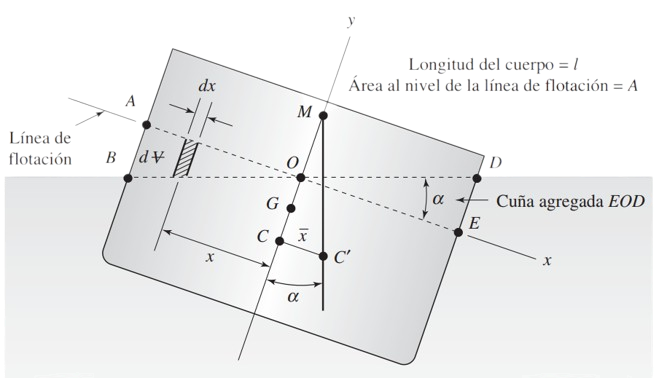
\includegraphics[width=\linewidth]{estabilidad}
			agreguen si falta...
		\end{cajita}
	\end{multicols}	
			
			
\end{document}